\documentclass[fontsize=11pt,a4paper,oneside]{scrartcl}

% ---- Sprache und Textformatierung ----
\usepackage{fontspec}
\usepackage{polyglossia}
\setdefaultlanguage{english}
\usepackage{microtype}
\usepackage{acronym}

% ---- KOMA-Script Seiteneinstellungen ----
\usepackage[onehalfspacing]{setspace}  
\usepackage[headsepline]{scrlayer-scrpage}
\usepackage{csquotes}
\usepackage{nowidow}

% Kopfzeilen-Konfiguration
\clearpairofpagestyles  % Alle bestehenden Kopf- und Fußzeilen löschen
\addtokomafont{pagehead}{\normalfont\small}  % Schriftart der Kopfzeile
\automark[section]{section}
\ihead{\textsc{\headmark}} 
\cfoot{\pagemark}

% ---- Mathematik und Symbole ----
\usepackage{amsmath, amsthm, amssymb, mathtools}
\usepackage[version=4]{mhchem}
\usepackage{chemformula}
\newcommand{\angstrom}{\text{\normalfont\AA}}

% ---- Graphische Pakete ----
\usepackage{xcolor}
\usepackage{graphicx}
\usepackage{float}
\usepackage{siunitx}
\usepackage{textpos}
\usepackage{subfig}
\usepackage{multirow}
\usepackage{booktabs}
\usepackage{chemfig}

% ---- Text-Positionierung ----
\usepackage[pscoord]{eso-pic}
\newcommand{\placetextbox}[3]{% \placetextbox{<horizontal pos>}{<vertical pos>}{<stuff>}
  \setbox0=\hbox{#3}% Put <stuff> in a box
  \AddToShipoutPictureFG*{% Add <stuff> to current page foreground
    \put(\LenToUnit{#1\paperwidth},\LenToUnit{#2\paperheight}){\vtop{{\null}\makebox[0pt][c]{#3}}}%
  }%
}%

% ---- Bibliographie ----
\usepackage[backend=biber,
    citestyle=numeric-comp,
    bibstyle=numeric, 
    sorting=none,
    autocite=superscript,
    bibwarn=true,
    isbn=false,
    url=false,
    eprint=false,
    doi=false
]{biblatex}

% Bibliographie-Dateien
\addbibresource{/Users/lucashirschfeld/sciebo/VsCode/LaTeX-Projects/bibliography/zotero.bib}

% Definition eines neuen Zitierbefehls mit eckigen Klammern
\DeclareCiteCommand{\supercite}[\mkbibsuperscript]%
    {\usebibmacro{cite:init}%
        \let\multicitedelim\supercitedelim%
        \iffieldundef{prenote}%
        {}%
        {\BibliographyWarning{Ignoring prenote argument}}%
        \iffieldundef{postnote}%
        {}%
        {\BibliographyWarning{Ignoring postnote argument}}%
        \bibleftbracket}%
    {\usebibmacro{citeindex}%
        \usebibmacro{cite:comp}}%
    {}%
    {\usebibmacro{cite:dump}%
        \bibrightbracket}

% ---- Hyperlinks ----
\usepackage{hyperref}
\hypersetup{colorlinks=true, linkcolor=black, citecolor=black, urlcolor=black}

% ---- Dokumenteinstellungen ----
\newcommand{\mylinespread}{1.5}
\setlength{\parindent}{0em}
\setlength{\parskip}{1em}

% ---- Metadaten ----
\def\Autor{Lucas Hirschfeld, s6luhirs@uni-bonn.de}
\def\Titel{QC II - Part 2: Application}
\def\Date{First Submission: \today}
\def\PiC{Supervisor: Benedikt Bädorf, Robin Dahl}
\def\Abstract{} 

\begin{document}
\pagestyle{empty}
\begin{titlepage}
    \begin{center}
        \vspace*{\fill}
        {\LARGE\bfseries \Titel}\par\vspace{2cm}
        {\Autor\par\vspace{0.5cm}\PiC\par\vspace{1cm}\par\vspace{0.2cm}\Date\par\vspace{5cm}}
    \end{center}
    {\Abstract\vspace{0.5cm}\par}\vfill
\end{titlepage}

\pagestyle{scrheadings}
\tableofcontents
\pagenumbering{arabic}
\clearpage


\section{Electron Correlation}

\subsection{Multireference Methods}

The dissociation of \ac{HF} was studied using different methods for H-F bond distances between 0.5~\AA{} and 4.0~\AA{} using the def2-TVZP basis set. The calculation was done using ORCA 5.0.4 \autocite{Neese2012,Neese2022}. The following methods were used: \ac{RHF}, \ac{UHF}, \ac{MP2}, \ac{CCSD(T)}, \acs{CASSCF}(2,2) and \acs{CASSCF}(6,6). \Acf{CASSCF}\autocite{Roos1980} is a multireference method that was used in two different ways, first with two active electrons in two active orbitals (CASSCF(2,2)) and second with six active electrons in six active orbitals (CASSCF(6,6)).

\autoref{fig:multireference} shows the dissociation curves for the different methods. The calculated energies are calculated relative to the dissociation limit of the H-F molecule. The dissociation limit is defined as the energy of a hydrogen atom and a fluorine atom at infinite distance.

\begin{figure}[htbp]
    \centering
    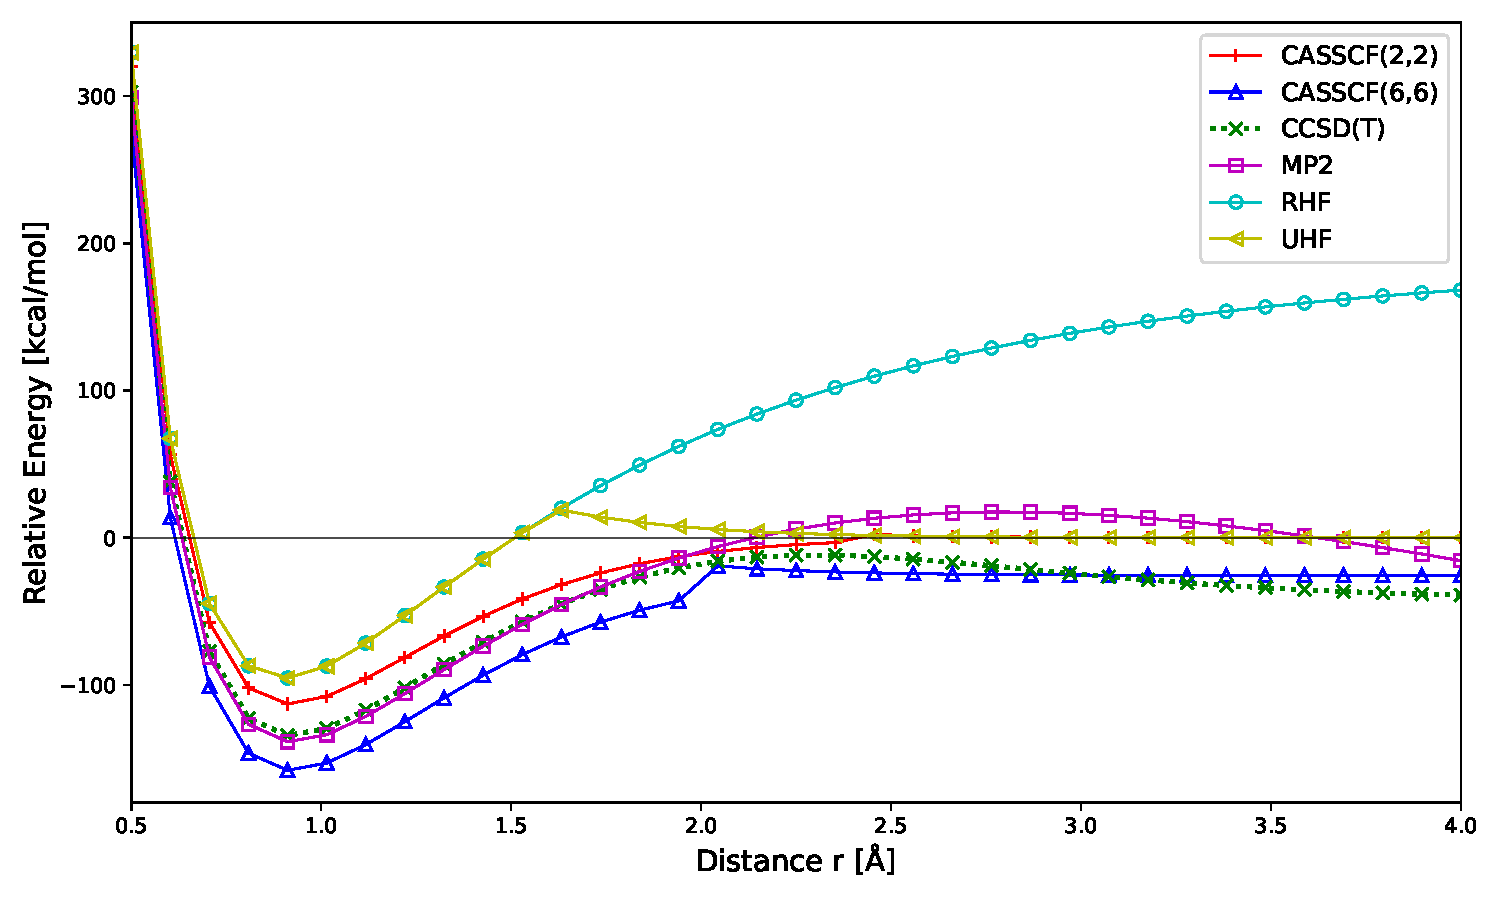
\includegraphics[width=0.95\textwidth]{images/ex1.pdf}
    \caption{H-F Dissociation for various methods.}
    \label{fig:multireference}
\end{figure}

The \ac{RHF} and \ac{UHF} methods show a dissociation curve that is not suitable for describing the dissociation of H-F. The \ac{RHF} curve approaches relative energies larger than 0~kcal/mol, which is not physically meaningful. This is due to the problem that each pair of electrons needs to occupy the same spatial wave function. As a result of this, the ionic dissociation of H-F is not described correctly.

This problem is absent in the \ac{UHF} curve, showing the correct dissociation limit. To obtain the best possible of the \ac{UHF} curve, the calculation was done from 0.5~\AA{} to 4.0~\AA{} and from 4.0~\AA{} to 0.5~\AA{} and the lowest energy was taken for each distance. Nevertheless, the \ac{UHF} curve shows a unphysical behaviour at 1.6~\AA{}, where the relative energy has a maximum. This is due to the fact that the \ac{UHF} method does not account for the electron correlation in the dissociation limit, which is caused by the way of how the calculation is done. Furthermore, both \ac{RHF} and \ac{UHF} methods calculate a binding energy at the equilibrium that is too low due to missing electron correlation.

Post \ac{HF} methods like \ac{MP2} and \ac{CCSD(T)} show a much better description of the dissociation of H-F, because they take the correlation effects into account. The \ac{MP2} energy correction is calculated as follows:


\begin{equation}
        E_0^{(2)}= \frac{1}{4} \sum_{i,j,ab} \frac{| \langle ij || ab \rangle| ^2 }{\epsilon_i + \epsilon_j - \epsilon_a - \epsilon_b},
        \label{eq:mp2_energy}
\end{equation}

where $\langle ij || ab \rangle$ are the two-electron integrals and $\epsilon_i$, $\epsilon_j$, $\epsilon_a$ and $\epsilon_b$ are the orbital energies of the occupied and virtual orbitals. However, this results that the \ac{MP2} energy correction approaches $- \infty$ for large distances, which is not physically meaningful. This occurs because the energy difference between occupied and virtual orbitals decreases for large distances, which leads to denominator approaching zero. A similar argument can be made to a lesser extent regarding \ac{CCSD(T)}, given the perturbative calculation of triple excitations.

Both \ac{CASSCF} methods describe the dissociation of H-F correctly, but have an unphysical behavior at 2.5~\AA{} for the \ac{CASSCF}(2,2) and at 2.0~\AA{} for the \ac{CASSCF}(6,6) method, which is not as drastic as in the \ac{UHF} curve. The \ac{CASSCF}(2,2) method computed to high energies at the equilibrium distance, but the description of the dissociation limit is accurate with only 2 active electrons in 2 active orbitals.

\clearpage
\subsection{Carbenes}

The calculation of the singlet-triplet energy splitting $\Delta E_{S-T}$ for two carbenes, namely Methylene and \textit{p}-Benzyne, and the Methylene H-C-H angles $\alpha_\mathrm{HCH}$ were computed using the def2-TZVP basis set and the following methods: \ac{HF}, \ac{MP2}, \ac{CCSD(T)}, \ac{B3LYP}, \ac{TPSS} and \ac{PW6B95}. The geometries for the \ac{CCSD(T)} calculations were optimized using the \ac{MP2} method in a def2-TZVP basis set. The structure of the carbenes is shown in \autoref{fig:carbenes}.

\begin{figure}[htbp]
    \centering
    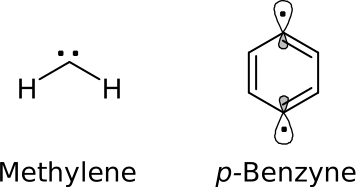
\includegraphics[width=0.4\textwidth]{images/carbenes.png}
    \caption{Structure of Methylene (left) and \textit{p}-benzyne (right). Figure taken from \cite{AKGrimme2025}.}
    \label{fig:carbenes}
\end{figure}

The calcuulations for the geometry optimizations and the single point calculations were done using TURBOMOLE \autocite{Turbomole2007}. The results for the singlet-triplet energy splitting $\Delta E_{S-T}$ and the Methylene H-C-H angles $\alpha_\mathrm{HCH}$ are shown in \autoref{tab:carbenes}.

\begin{table}[htbp]
    \centering
    \caption{Singlet-Triplet energy splittings (kcal/mol) for p-benzyne and methylene along methylene H-C-H angles. All values were obtained using a def2-TZVP basis. CCSD(T) calculations were performed using MP2 geometries.}
    \label{tab:carbenes}
        \begin{tabular}{@{}lcccc@{}} \toprule
        \multirow{2}{*}{Method} & \multicolumn{2}{c}{$\Delta E_{S-T} [\si{kcal/mol}]$} & \multicolumn{2}{c}{$\alpha_\mathrm{HCH}$} \\
        \cmidrule{2-3} \cmidrule{4-5}
        & p-Benzyne & Methylene & Singlet & Triplet \\
        \midrule
        HF & 80.4 & 28.4 & 103.7\textdegree & 131.8\textdegree \\
        MP2 & -28.6 & 15.8 & 102.4\textdegree & 133.1\textdegree \\
        CCSD(T) & -3.3 & 10.8 & - & - \\
        B3LYP & 13.4 & 11.9 & 101.9\textdegree & 135.1\textdegree \\
        TPSS & 7.0 & 17.8 & 101.3\textdegree & 135.4\textdegree \\
        PW6B95 & 14.3 & 12.6 & 101.6\textdegree & 134.8\textdegree \\
        \hline
        Experiment & -4.2 & 9.0 & 102.4\textdegree & 135.5\textdegree \\
        \bottomrule
        \end{tabular}
\end{table}

The only method that describes the singlet-triplet energy splitting $\Delta E_{S-T}$ with almost chemical accuracy (1~kcal/mol) for both systems is \ac{CCSD(T)}. The other methods show larger deviations from the experimental values. \ac{HF} overestimamtes the singlet-triplet energy splitting for both systems and results in too large $\Delta E_{S-T}$ values. This is due to the fact that a triplet needs to be calculated using \ac{UHF}, which contains spin contamination and therefore lowers the energy.

\ac{MP2} underestimates the $\Delta E_{S-T}$ for p-benzyne and overestimates the $\Delta E_{S-T}$ for methylene. Nevertheless, \ac{MP2} is the only method that describes the singlet-triplet energy splitting for p-benzyne with a negative value, which is in line with the experimental value and also gives a reasonable value for the $\Delta E_{S-T}$ of methylene. The large error in the p-benzyne $\Delta E_{S-T}$ is due to the small HOMO-LUMO gap, which leads to a large energy correction of the correlation energy (see \autoref{eq:mp2_energy}).

All the other methods show positive values for the singlet-triplet energy splitting $\Delta E_{S-T}$ of p-benzyne, which are not physically meaningful.

The H-C-H angles for methylene are also affected by the choice of method, but all methods predict a similar results for the angle and are in good agreement with the experimental values. It is to be noted that the angles for \ac{HF} again have the largest deviations from the experimental values.


\clearpage
\section{Basis Set Convergence}

The convergence of different basis sets is an important aspect of quantum chemical calculations. In this report, the basis set convergence of the formic acid dimer is investigated. The structure of the formic acid monomer and dimer are shown in \autoref{fig:monomer_dimer} and were optimized using the \ac{TPSS}-D3/def2-TZVP level of theory.

\begin{figure}[htbp]
    \centering
    \subfloat[Monomer]{%
        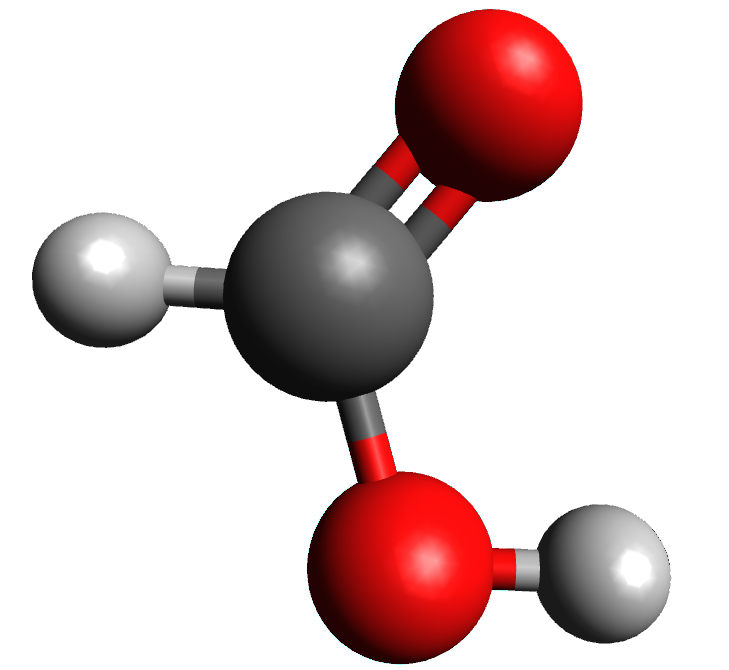
\includegraphics[width=0.32\textwidth]{images/monomer.png}
    }
    \hfill
    \subfloat[Dimer]{%
        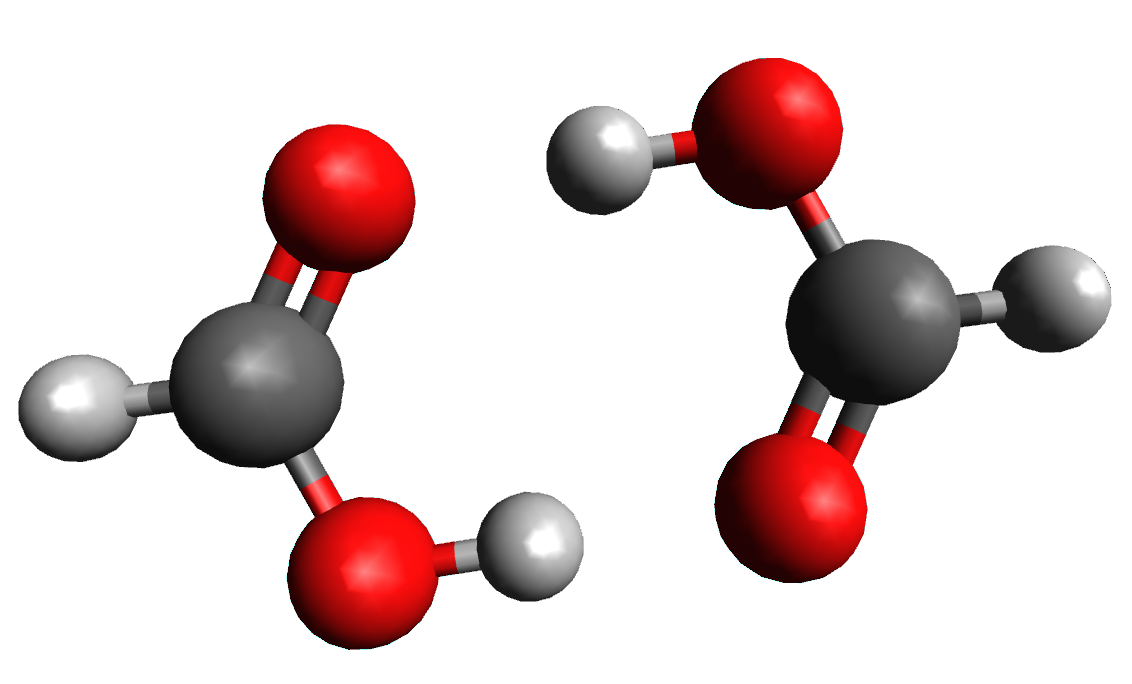
\includegraphics[width=0.6\textwidth]{images/dimer.png}
    }
    \caption{Monomer and dimer structures for formic acid. Geometries were optimized on the \ac{TPSS}-D3/def2-TZVP level of theory.}
    \label{fig:monomer_dimer}
\end{figure}

The dimerization energy of formic acid is defined as the difference between the dimer energy and the sum of the monomer energies:

\begin{equation}
    \Delta E_\mathrm{dimerization} = E_\mathrm{dimer} - 2\cdot E_\mathrm{monomer},
    \label{eq:dimerization_energy}
\end{equation}

where $E_\mathrm{dimer}$ is the energy of the dimer and $E_\mathrm{monomer}$ is the energy of the monomer.

The dimerization energy was computed for three different methods, namely \ac{HF}, \ac{MP2} and \ac{TPSS}-D3, using the cc-pVXZ\autocite{Dunning1989} and aug-cc-PVXZ basis sets, where X = D, T, Q. The dimerization energy was computed for each method and basis set combination with optimized geometries at the \ac{TPSS}-D3/def2-TZVP level. The results are shown in \autoref{fig:basis_convergence}.

\begin{figure}[htbp]
    \centering
    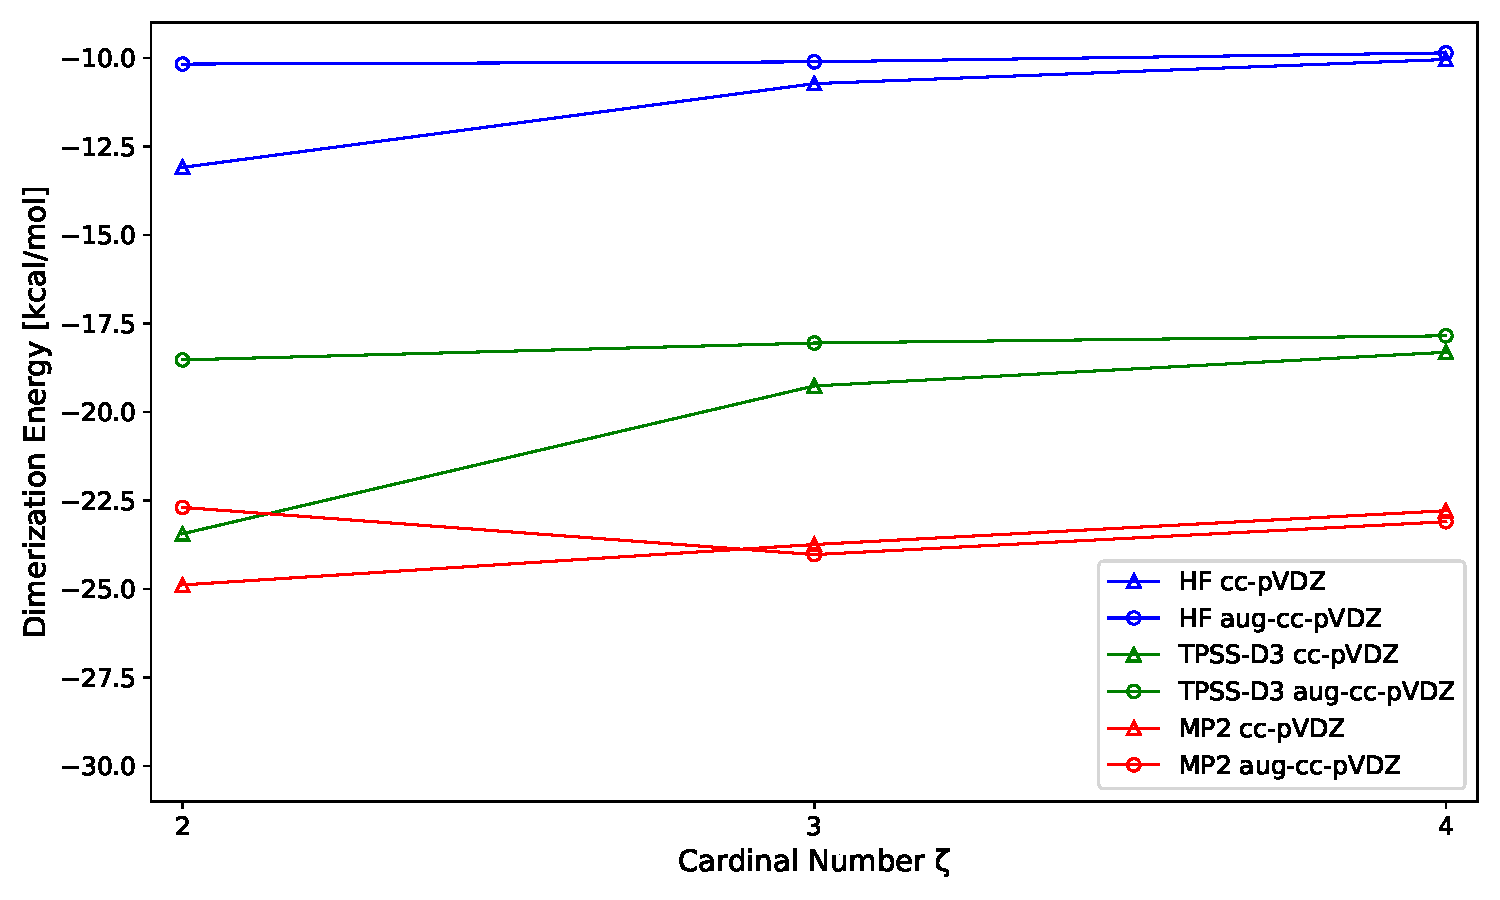
\includegraphics[width=0.95\textwidth]{images/ex2.pdf}
    \caption{Convergence behaviour for the formic acid dimer aug-cc-PVXZ and cc-pVXZ basis sets at \ac{HF}, \ac{MP2}, and \ac{TPSS}-D3 levels of theory.}
    \label{fig:basis_convergence}
\end{figure}

The dimerization energy for formic acid shows a strong dependence on the choice of basis set and method. The aug-cc-PVXZ basis sets generally yield more negative dimerization energies compared to the cc-pVXZ basis sets. For a cardinal number of four, all methods and basis sets are at similar dimerization energies.

The calculations generally contains two different errors, the \ac{BSIE} and the \ac{BSSE}. The \ac{BSIE} is the error that arises from the finite size of the basis set and is the difference between the \ac{CBS} limit and the energy computed with a finite basis set. This error is always present and not only limited to dimerization energies. The \ac{BSIE} can be reduced by using larger basis sets, but it is not possible to eliminate it completely. It is important to note that the convergence with respect to the basis set depends on the used method. For instance, SCF energies converge exponentially with respect to the basis set size, while correlation energies converge with inverse cubic behavior.

The \ac{BSSE} is the error that arises from the interaction of the basis functions of the two monomers in the dimer. This error is present in energies for the dimer or other intramolecular interactions. The \ac{BSSE} is generally larger for an increased basis sets, because the interaction between the basis functions of the two monomers is stronger. The \ac{BSSE} compensates the \ac{BSIE} and leads to a artificially lowered dimerization energy. The \ac{BSSE} is only not present if one uses a minimal basis set, which is not the case here.

Both errors can be reduced by using larger basis sets, but it is not possible to eliminate them completely, only by theoretically using a \ac{CBS}. Another possibility is the use of Boys-Bernardi counterpoise correction, which is a method to correct for the \ac{BSSE}.

\clearpage
\section{Thermochemistry}

The reaction enthalpies $\Delta H$ for the Haber-Bosch process and the steam-reforming of methane were computed using the different level of theory.

\begin{center}
    \chemfig{N_2 + 3H_2 \rightarrow 2NH_3}

    \chemfig{CH_4 + H_2O \rightarrow CO + 3H_2}
\end{center}

The geometries were optimized on the \ac{TPSS}-D3/def2-TZVP level of theory. In addition, the geometries of the molecules involved in the Haber Bosch process were also optimized at the \ac{MP2}/def2-TZVP level of theory and the  RMSD to the \ac{TPSS}-D3/def2-TZVP geometries was computed. The results are shown in \autoref{tab:rmsd}. The RMSD values are in the order of $10^{-3}$~\AA{} and show that the geometries are very similar. This indicates that the choice of the method does not have a large impact on the geometry and the selection of the method can mainly be based on the computational cost.

\begin{table}[htbp]
    \centering
    \caption{RMSD between \ac{TPSS}-D3 and \ac{MP2} geometries optimized in a def2-TZVP basis for all molecules involved in the Haber-Bosch process.}
    \label{tab:rmsd}
        \begin{tabular}{@{}lc@{}} \toprule
        & RMSD (\AA) \\ \midrule
        N$_2$ & $5.67 \cdot 10^{-3}$ \\
        H$_2$ & $3.06 \cdot 10^{-3}$ \\
        NH$_3$ & $6.58 \cdot 10^{-3}$ \\ \bottomrule
        \end{tabular}
\end{table}

The reaction enthalpies of both reactions were computed using the \ac{MP2} and \ac{B3LYP}-D3 methods in a def2-TZVP basis set and The \ac{B2PLYP}-D3 and \ac{CCSD(T)} in a def2-QZVP basis set. First, the single point energies were computed using the optimized geometries from the \ac{TPSS}-D3/def2-TZVP level of theory. The single point energies were then corrected for the thermal corrections at 298 K. The results are shown in \autoref{tab:thermochemistry}.

\begin{table}[htbp]
    \centering
    \caption{Reaction enthalpies in kcal/mol for the Haber-Bosch process and steam-reforming of methane. Geometries were optimized on the \ac{TPSS}-D3/def2-TZVP level. \ac{B2PLYP}-D3 and \ac{CCSD(T)} energies were computed in a def2-QZVP basis, def2-TZVP was used for all other methods.}
    \label{tab:thermochemistry}
        \begin{tabular}{@{}lcccc@{}} \toprule
        Reaction & \ac{MP2} & \ac{B3LYP}-D3 & \ac{B2PLYP}-D3 & \ac{CCSD(T)} \\ \midrule
        \multirow{2}{*}{Haber-Bosch} & -12.1 & -21.0 & -23.9 & -24.5 \\ \cmidrule{2-5}
        & \multicolumn{4}{c}{Exp\autocite{AKGrimme2025}: -22.5} \\ \midrule
        \multirow{2}{*}{Steam-Reforming} & 43.1 & 47.3 & 50.4 & 51.4 \\ \cmidrule{2-5}  
        & \multicolumn{4}{c}{Exp\autocite{AKGrimme2025}: 49.3} \\ \bottomrule
        \end{tabular}
\end{table}

In total, all methods yield a reasonable reaction enthalpies. The \ac{MP2} and the \ac{B3LYP}-D3 methods underestimate the reaction enthalpies for both reactions, while the \ac{B2PLYP}-D3 and \ac{CCSD(T)} methods overestimate them.

The \ac{B2PLYP}-D3 method yields the best agreement with the experimental values for both reactions, while the \ac{CCSD(T)} method is slightly worse. The \ac{MP2} and \ac{B3LYP}-D3 methods are not as accurate.

The general trend of the \textit{Jacob's Ladder} is observed for this example, where the more accurate methods yield better results. The hybrid functional \ac{B3LYP}-D3 is more accurate than the pure \ac{MP2} method, but not as accurate as the double hybrid \ac{B2PLYP}-D3.

\clearpage
\section{Kinetics}

The kinetic isotope effect for the reaction of methane with a hydroxyl radical was studied using the \ac{B3LYP}-D3\autocite{Becke1993}/def2-TZVP level of theory for a transition state search, which was performed using TURBOMOLE\autocite{Turbomole2007}.

The transition state research was done for \ce{CH4-OH} and \ce{CD4-OH}, where the latter is the deuteriated isotopologue of methane. The geometry of the transition state is shown in \autoref{fig:kinetics}.

\begin{figure}[htbp]
    \centering
    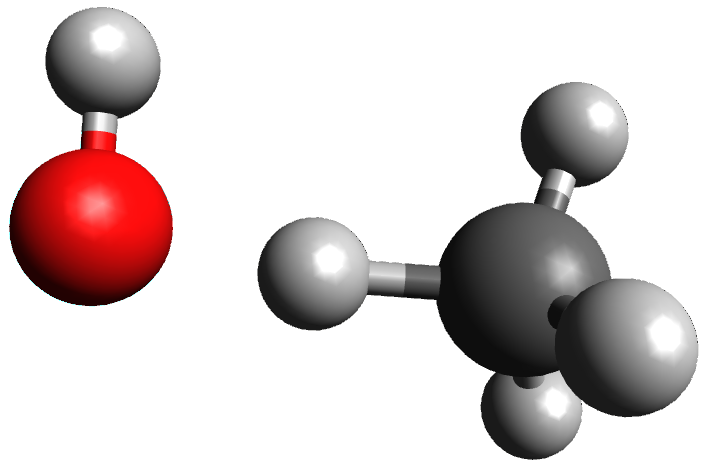
\includegraphics[width=0.6\textwidth]{images/ch4oh.png}
    \caption{Geometry of the transition state for the reaction of methane with a hydroxy radical. The transition state was optimized on the \ac{B3LYP}-D3/def2-TZVP level of theory.}
    \label{fig:kinetics}
\end{figure}

The electronic energies, \ac{ZPVE} and thermal corrections at 298 K for the reactants and transition states are shown in \autoref{tab:kinetics}. The electronic energies were computed using the \ac{B3LYP}-D3/def2-TZVP level of theory. The \ac{ZPVE} and thermal corrections were computed using the same level of theory.

\begin{table}[htbp]
    \centering
    \caption{Electronic energies (E$_h$) along with zero-point vibrational energies and thermal corrections (298 K) for reactants and transition states.}
    \label{tab:kinetics}
        \begin{tabular}{@{}lccccc@{}} \toprule
        & CH$_4$ & CD$_4$ & OH & CH$_4$ - OH & CD$_4$ - OH \\ \midrule
        $E_\mathrm{el}$ [kcal/mol] & -25.415 & -25.415 & -47.524 & -72.937 & -72.937 \\
        ZPVE (kcal/mol) & 27.959 & 20.500 & 5.256 & 31.749 & 25.217 \\
        Thermal correction (kcal/mol) & 2.393 & 2.468 & 2.074 & 3.475 & 3.732 \\ \bottomrule
        \end{tabular}
\end{table}

The energies in \autoref{tab:kinetics} amount to

\begin{center}
    $\Delta H_H^{\ddagger} = 0.325$ kcal/mol

    $\Delta H_D^{\ddagger} = 1.434$ kcal/mol
\end{center}

with the subscripts H and D referring to regular and deuteriated methane respectively.

As seen in \autoref{tab:kinetics}, the transition state for the reaction of methane with a hydroxy radical is lower in energy than the transition state for the reaction of deuteriated methane with a hydroxy radical due to the fact that the \ac{ZPVE} and the thermal corrections are lower for the regular methane. The electronic energies are the same for both transition states, because they do not depend on the mass of the nuclei in the molecules, as long as relativistic effects are not neglected.

The thermal corrections in contrast depend on the mass of the nuclei, which is why the thermal correction for the transition state of deuteriated methane is larger than for regular methane. The vibrational frequencies, which are taken in account for the thermal correction, can be computed from the harmonic oscillator model:

\begin{equation}
    \nu = \frac{1}{2\pi} \sqrt{\frac{k}{\mu}},
\end{equation}

where $k$ is the force constant and $\mu$ is the reduced mass of the system. The reduced mass can be computed from the masses of the two atoms involved in the reaction:

\begin{equation}
    \mu = \frac{m_1 \cdot m_2}{m_1 + m_2}.
\end{equation}

The reduced mass for the transition state of regular methane is smaller than for the transition state of deuteriated methane, which leads to larger vibrational frequencies and therefore a smaller thermal correction.

The relative reaction rates can then be determined from $\Delta H^{\ddagger}$ according to:

\begin{equation}
    \frac{k_H}{k_D} = \exp\left(\frac{\Delta H_D^{\ddagger} - \Delta H_H^{\ddagger}}{RT}\right) = 6.502
\end{equation}

This indicates that the reaction of methane with a hydroxy radical is about 6.5 times faster than the reaction of deuteriated methane with a hydroxy radical.

\clearpage
\section{Solvation}

The S$_\mathrm{N}$2 reaction of chloromethane with fluoride is a well-known reaction in organic chemistry. The reaction proceeds via a transition state, where the nucleophile attacks the electrophile and the leaving group is expelled.

The solvation effects on the reaction can be significant, as the presence of a solvent can stabilize certain states and alter the reaction pathway. In this case, we consider the solvation effects of methanol on the S$_\mathrm{N}$2 reaction of chloromethane with fluoride. The geometry of the transition state in vacuum is shown in \autoref{fig:sn2_transition_state}.

\begin{figure}[htbp]
    \centering
    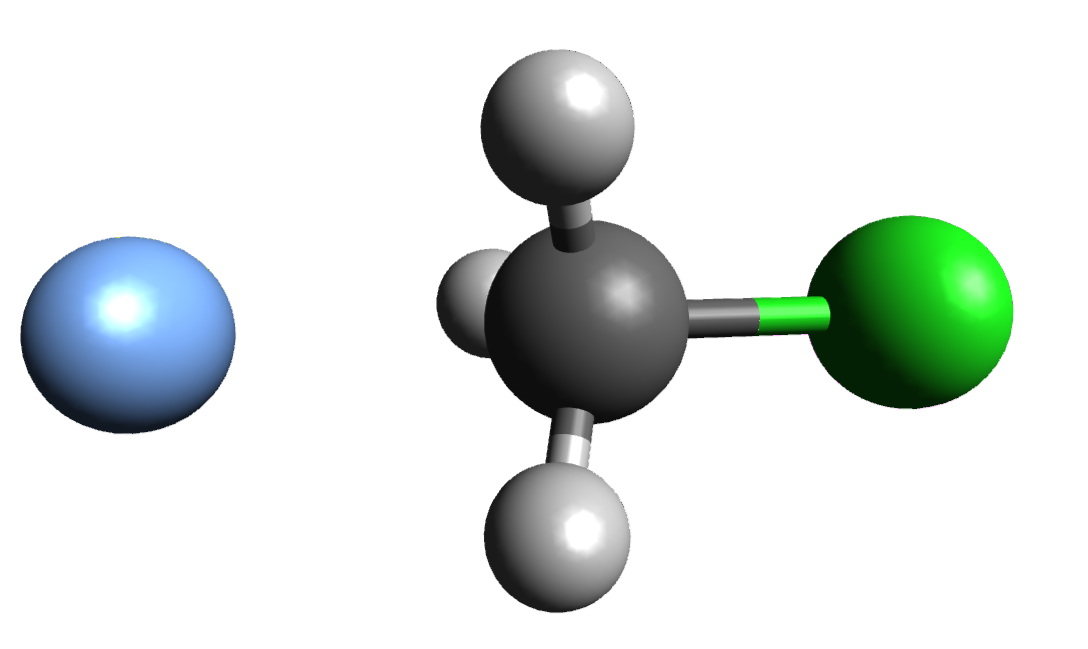
\includegraphics[width=0.6\textwidth]{images/ch3cl-f.png}
    \caption{Geometry of the transition state for the S$_\mathrm{N}$2 reaction of Chloromethane and Fluoride. The transition state was optimized on the \ac{PW6B95}-D3/def2-TZVP level of theory. The C-F distance in the figure is 4.00~\AA\ in vacuum.}
    \label{fig:sn2_transition_state}
\end{figure}

The potential energy curves for the S$_\mathrm{N}$2 reaction of chloromethane with fluoride in vacuum and in the presence of methanol as an implicit solvent were computed using the \ac{PW6B95}\autocite{Zhao2006}-D3\autocite{Grimme2011}/def2-TZVP\autocite{Weigend2023} level of theory. Both calculations were performed using TURBOMOLE\autocite{Turbomole2007}. The potential energy curves were computed for C-F distances between 2.25~\AA{} and 8.0~\AA{} in vacuum and in the presence of methanol as an implicit solvent using the COSMO model.
The potential energy curves are shown in \autoref{fig:sn2_solvation}.

\begin{figure}[htbp]
    \centering
    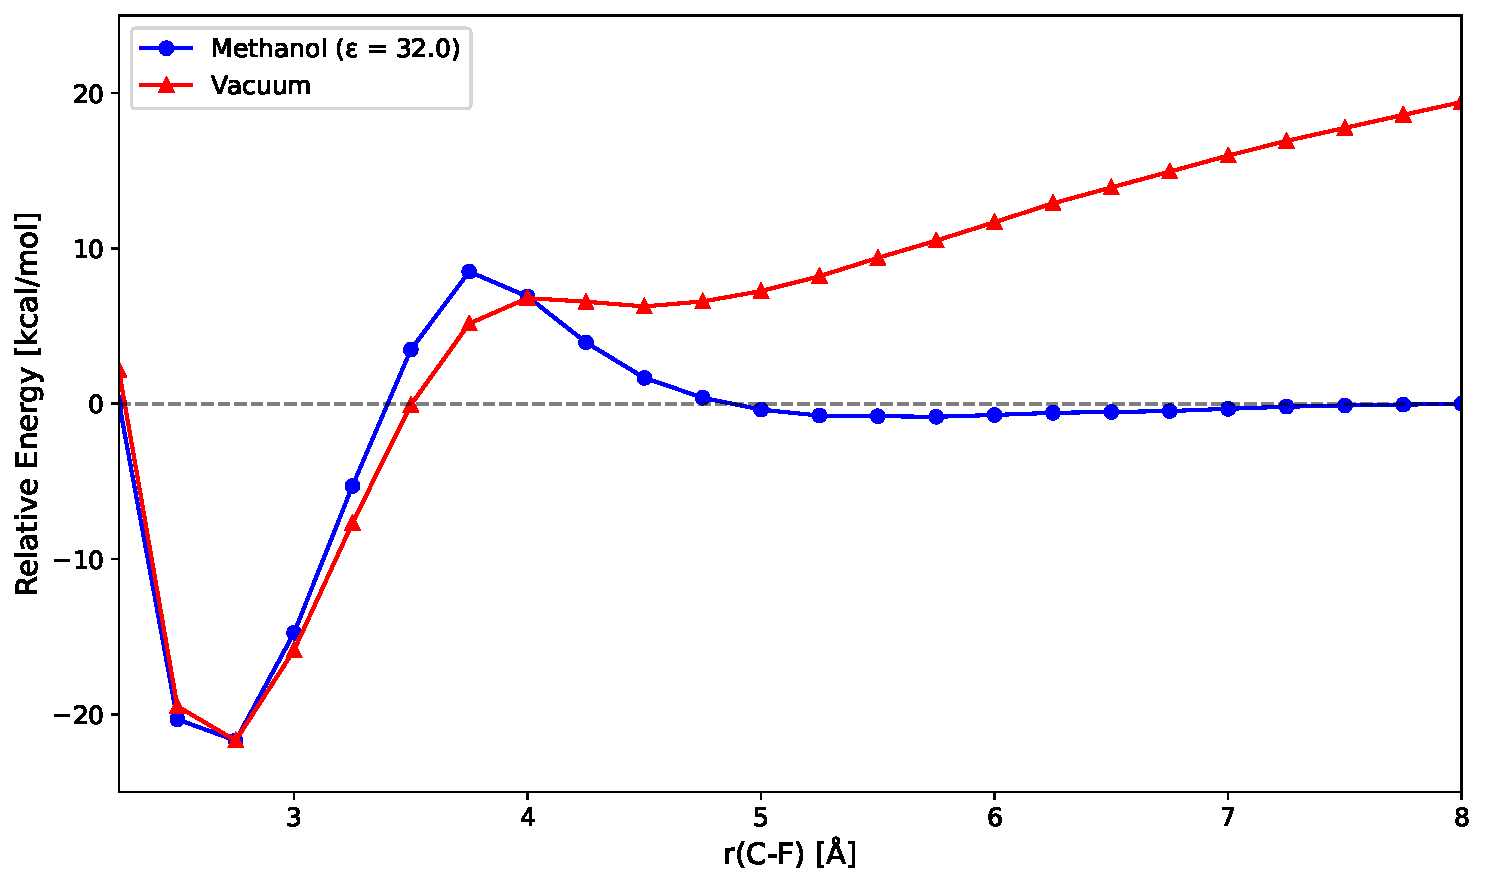
\includegraphics[width=0.95\textwidth]{images/ex5.pdf}
    \caption{Relative energy curve for the S$_\mathrm{N}$2 reaction of Chloromethane and Fluoride. Blue circles: In presence of methanol as an implicit solvent. Red triangles: In vacuum. The blue curve has been adjusted to the dissociation limit and the red curve was shifted such that both minima align.}
    \label{fig:sn2_solvation}
\end{figure}

The potential energy curves in \autoref{fig:sn2_solvation} show that the reaction proceeds via a transition state, where the C-F distance is about 3.75~\AA{} in vacuum and about 4.00~\AA{} in the presence of methanol as an implicit solvent. The transition state is lower in energy in the presence of methanol, which indicates that the solvation stabilizes the transition state and lowers the activation barrier for the reaction. The different C-F distances in vacuum and in the presence of methanol are due to the charge shielding effect of the solvent.

The reaction barriers for the reactions can be estimated based on the potential curves:

\begin{center}
    $\Delta E_\mathrm{solv}^{\ddagger} = 9.3$ kcal/mol

    $\Delta E_\mathrm{gas}^{\ddagger} = 0.5$ kcal/mol
\end{center}

The reaction barrier in the presence of methanol as an implicit solvent is significantly higher than in vacuum, which indicates that the solvation effects are significant and can alter the reaction pathway.

Nevertheless, the reaction barrier can not be compared this easy, because the fluoride ion in vacuum is not solvated, while the fluoride ion in the presence of methanol is solvated. The solvation of the fluoride ion in methanol leads to a stabilization of the fluoride ion, because the negative charge of the fluoride ion is shielded by the positive solvate molecules. In contrast, the fluoride ion in vacuum is not shielded and therefore unstable. As the distance between fluoride ion and the chloromethane molecule in vacuum decreases, the fluoride ion is stabilized by the chloromethane molecule. In the presence of methanol, the fluoride ion is already stabilized by the solvent and the energy curve converges towards the dissociation limit at a larger distance. This leads to a larger reaction barrier in the presence of methanol.


\clearpage
\section{Activation Energies}

The reaction path for the Claisen rearrangement of allyl-vinyl ether and the Diels-Alder reaction of cyclopentadiene to \textit{endo}-dicyclopentadiene were computed using the double ended \ac{GSM} at the GFN2-xTB\autocite{Bannwarth2019} level. First, geometries of the reactant and product were optimized using the GFN2-xTB method. Then, the double ended \ac{GSM} was used to compute the reaction path between the reactant and product of both reactions for 20 points. The reaction paths are shown in \autoref{fig:activation_energy_1} and \autoref{fig:activation_energy_2}.

\begin{figure}[htbp]
    \centering
    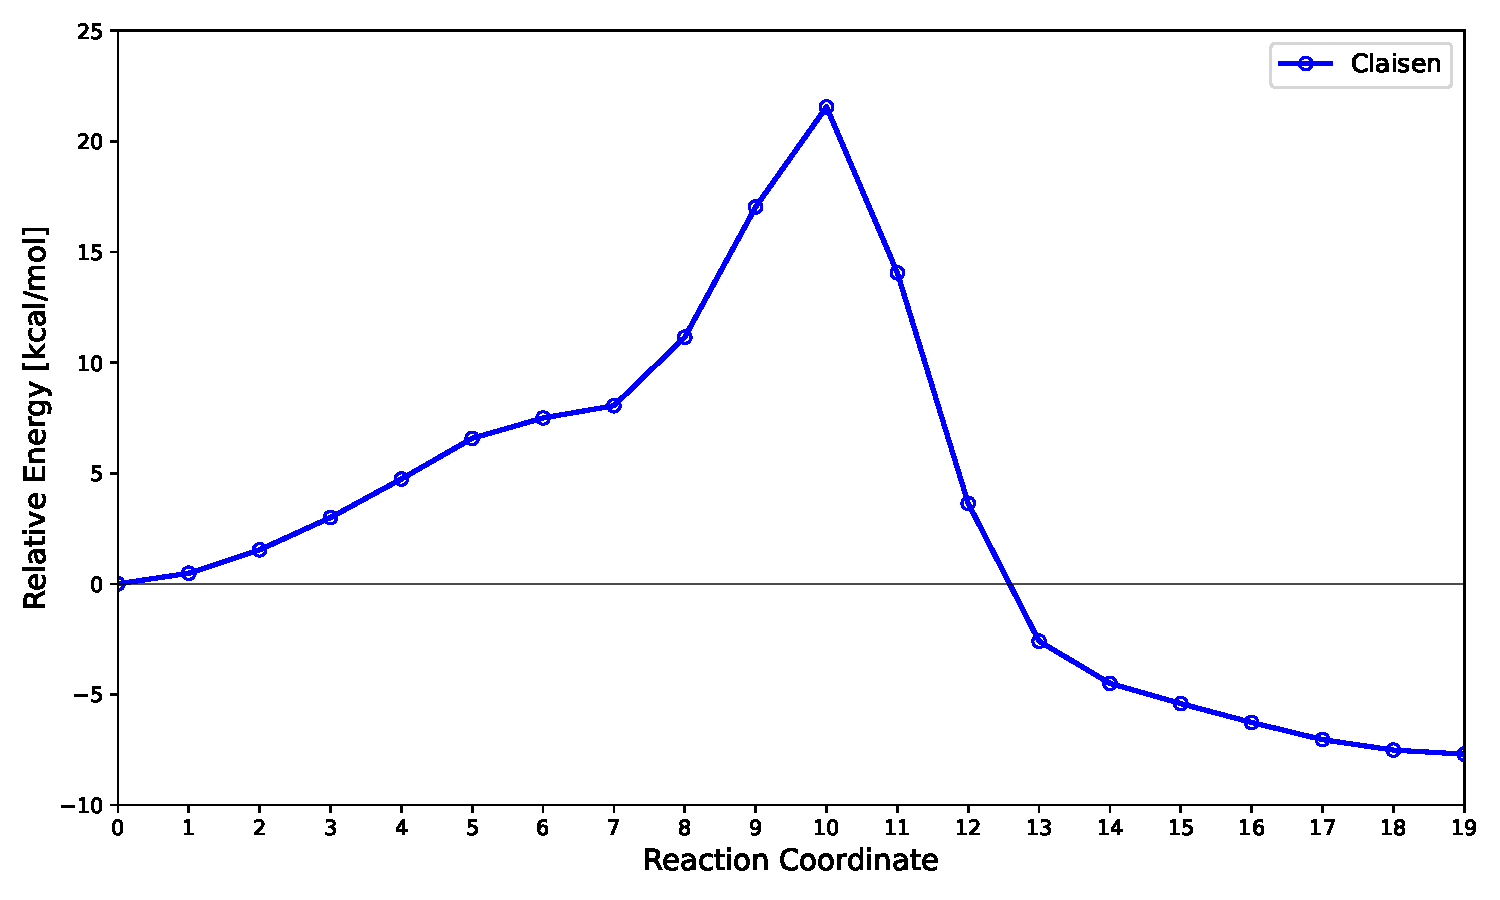
\includegraphics[width=0.8\textwidth]{images/ex6-1.pdf}
    \caption{Relative energy along the reaction coordinate for the Claisen rearrangement of allyl-vinyl ether.}
    \label{fig:activation_energy_1}
\end{figure}

The activation energy for the Claisen rearrangement of allyl-vinyl ether is about 21.6~kcal/mol. The reaction proceeds via a cyclic transition state, where the C-O bond is broken and the C-C bond is formed. The transition state is lower in energy than the reactant and product, which indicates that the reaction is exothermic.

This activation energy is smaller than the experimental value of 30.6~kcal/mol \autocite{Schuler1950}, which suggests that the computational method used may underestimate the activation energy. This indicates that the transition state is not described accurately enough, which can be due to the limitations of the GFN2-xTB method. The GFN2-xTB method is a semi-empirical method that is not as accurate as ab initio methods, but it is computationally efficient and can be used for larger systems.

\begin{figure}[htbp]
    \centering
    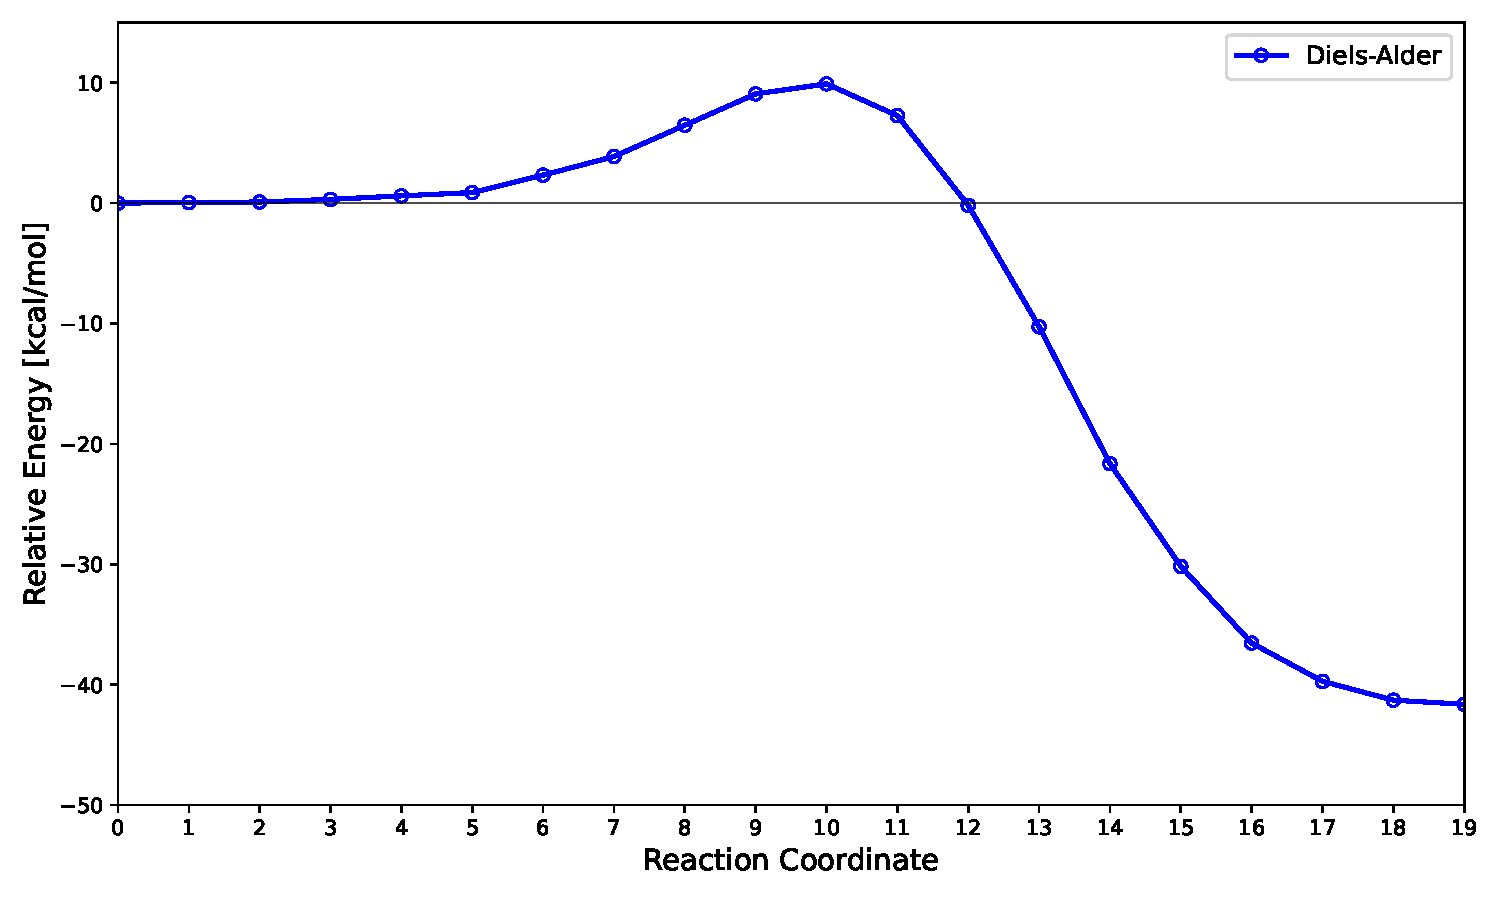
\includegraphics[width=0.8\textwidth]{images/ex6-2.pdf}
    \caption{Relative energy along the reaction coordinate for the Diels-Alder reaction of cyclopentadiene to \textit{endo}-dicyclopentadiene.}
    \label{fig:activation_energy_2}
\end{figure}

The activation energy for the Diels-Alder reaction of cyclopentadiene to \textit{endo}-dicyclopentadiene is about 9.9~kcal/mol. The reaction proceeds via a transition state, where the C-C bond is formed and the C=C bond is broken. The transition state is lower in energy than the reactant and product, which indicates that the reaction is exothermic.

The reliability of the activation energy for both reactions can be improved by using a higher level \ac{DFT} method. This would provide a more accurate description of the reaction path, but would also increase the computational cost. Furhter improvements can be made by optimizing the input geometries of the reactants and products, as this has a large impact on the used method.


\clearpage
\section{Noncovalent Interactions}

Noncovalent interactions are important in many chemical and biological processes. In this section, the interaction of methane with argon and krypton is investigated. The geometry of the methane-argon complex is shown in \autoref{fig:ng_ch4}.

\begin{figure}[htbp]
    \centering
    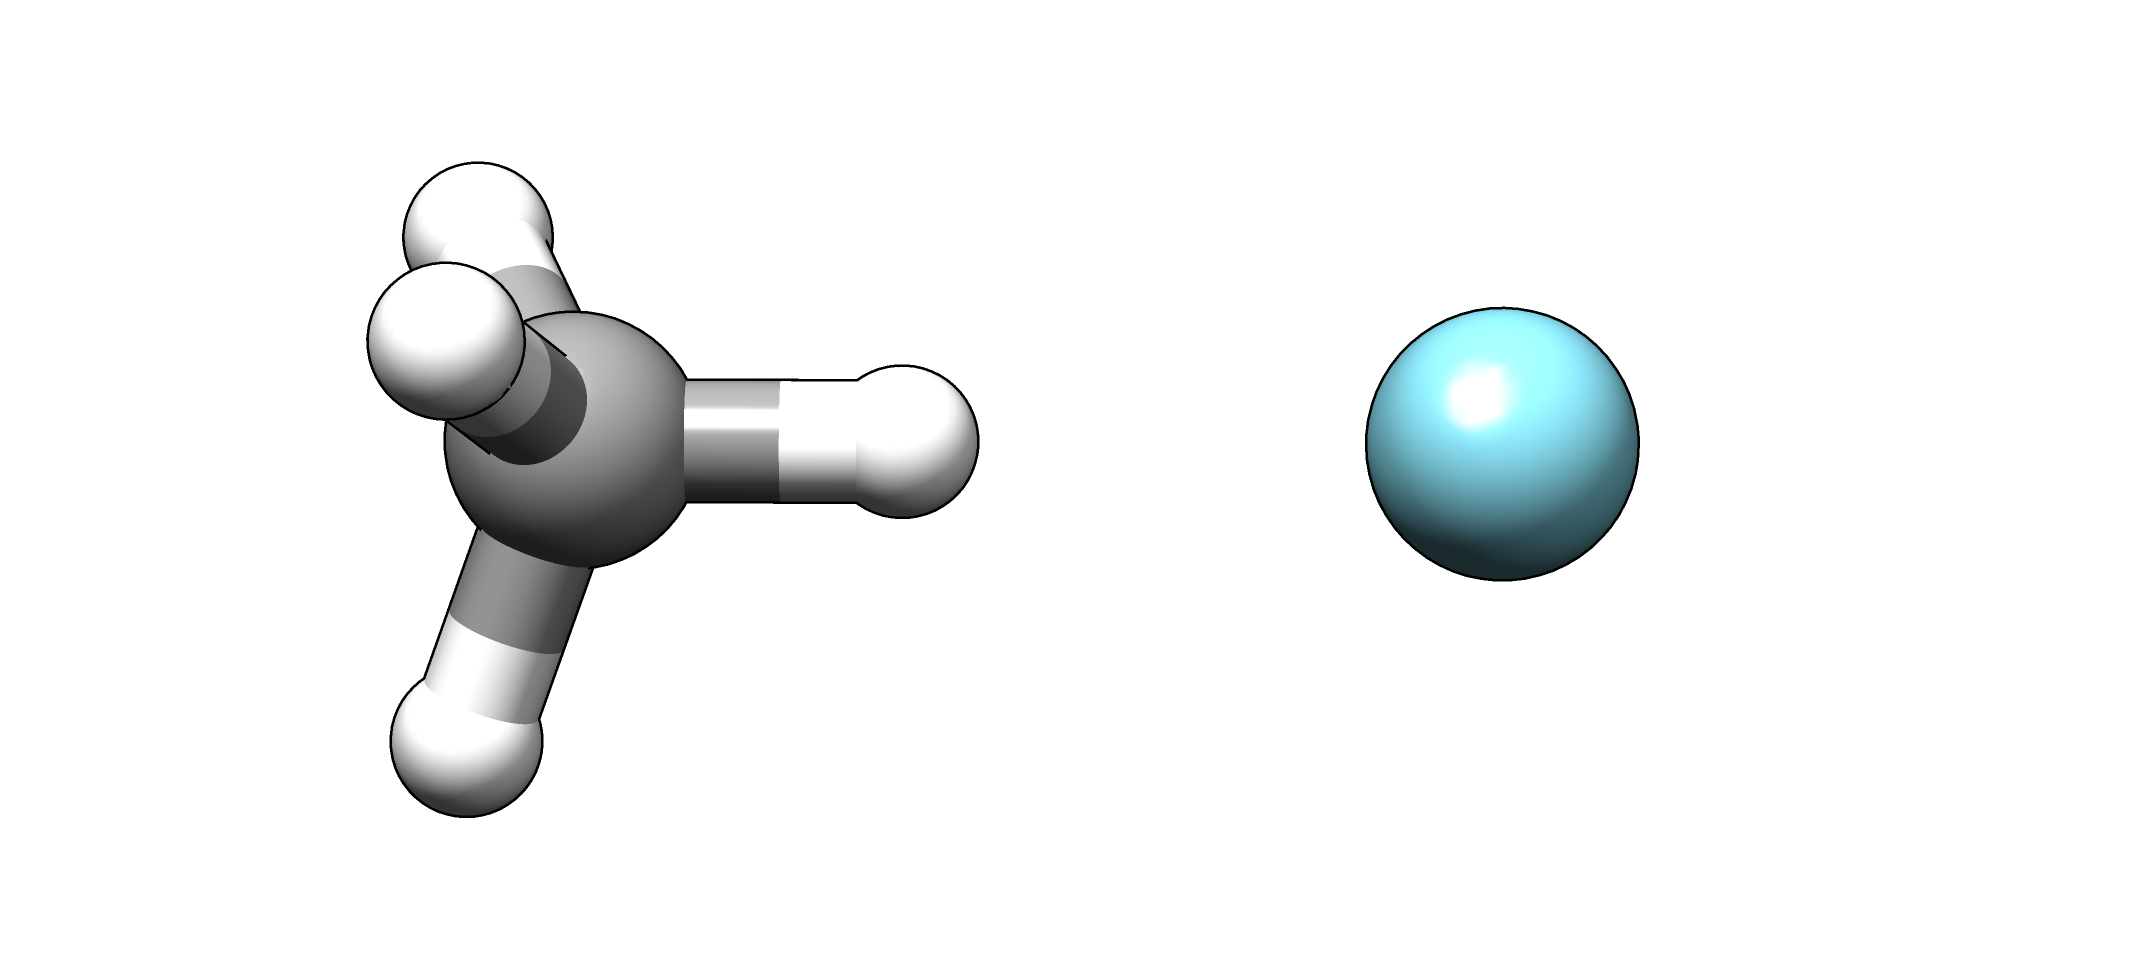
\includegraphics[width=0.7\textwidth]{images/ng_ch4.png}
    \caption{Geometry of the CH$_4 \cdot \cdot$ Ar compex. Figure taken from \cite{AKGrimme2025}.}
    \label{fig:ng_ch4}
\end{figure}

The potential energy curves for the interaction of methane with argon and krypton were computed using the following methods: \ac{BLYP}, \ac{BLYP}-D3 and \ac{MP2}. All calculations were performed using the def2-QZVP basis set. The potential energy curves were computed for CH$_4$-Ar/Kr distances between 4.5~\AA{} and 15.0~\AA{}, were normalized to the dissociation limit and are shown in \autoref{fig:noncovalent_interactions}.

\begin{figure}[htbp]
    \centering
    \subfloat[CH$_4 \cdots$Ar]{%
        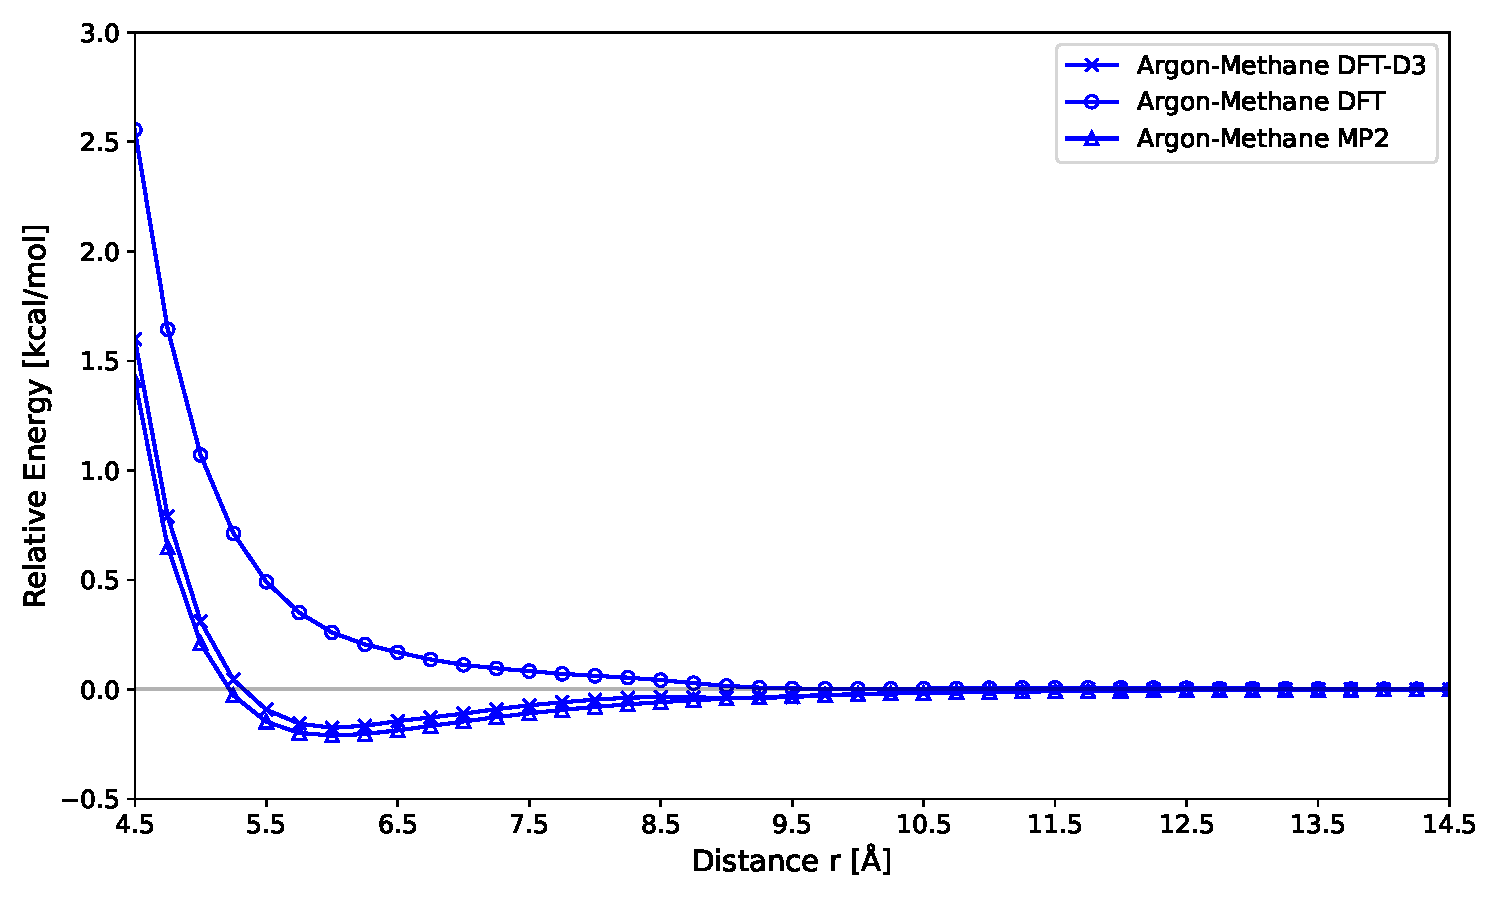
\includegraphics[width=0.8\textwidth]{images/ex7-1.pdf}
    }
    \hfill
    \subfloat[CH$_4 \cdots$Kr]{%
        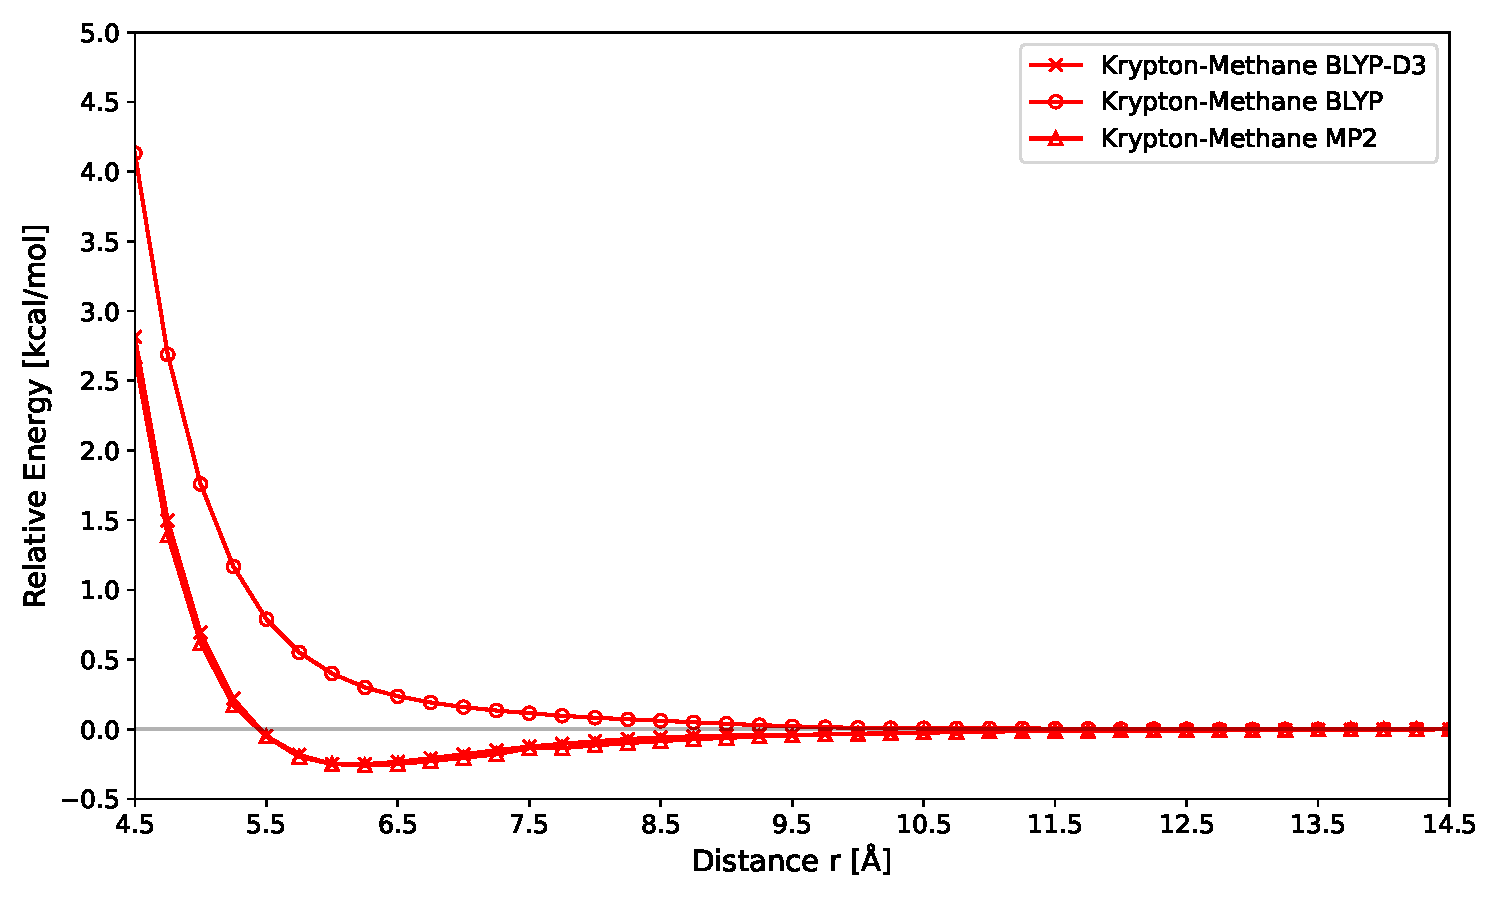
\includegraphics[width=0.8\textwidth]{images/ex7-2.pdf}
    }
    \caption{Potential energy curves for methane with argon (a) and krypton (b).}
    \label{fig:noncovalent_interactions}
\end{figure}

The potential energy curves in \autoref{fig:noncovalent_interactions} show the importance of dispersion interactions for noncovalent interactions. The \ac{BLYP} method does not account for dispersion interactions and therefore yields a repulsive potential energy curve, which is not physically meaningful.

The \ac{BLYP}-D3 method accounts for dispersion interactions and yields a potential energy curve that is in good agreement with the \ac{MP2} method. The \ac{MP2} method yields a potential energy curve that is slightly lower in energy than the \ac{BLYP}-D3 method. Both methods yield a minimum at around 6.0~\AA{} for the CH$_4$-Ar complex and for the CH$_4$-Kr complex.

\clearpage
\section{Spectroscopy}


\subsection{IR-Spectroscopy}

The IR-spectra of 1,4-Benzoquinone were computed on the \ac{TPSS}-D3/def2-SVP and \ac{HF}-D3/def2-SVP levels of theory using TURBOMOLE\autocite{Turbomole2007}. The structure of 1,4-Benzoquinone is shown in \autoref{fig:p_benzoquinone}.

\begin{figure}[htbp]
    \centering
    
\includegraphics[height=0.25\textwidth, angle=90]{images/P-Benzochinon.png}
    \caption{Structure of 1,4-Benzoquinone.}
    \label{fig:p_benzoquinone}
\end{figure}

First, the geometry of 1,4-Benzoquinone was optimized with TURBOMOLE\autocite{Turbomole2007} using the respective level of theory. Then, the vibrational modes were computed using the subprogram aoforce. The resulting IR-modes are shown in \autoref{tab:ir_spectrum}. Furthermore, the scaling factor for the IR-modes was calculated using the experimental values from \cite{AKGrimme2025} and the theoretical values from the \ac{TPSS}-D3/def2-SVP and \ac{HF}-D3/def2-SVP levels of theory. The scaling factor was calculated using the following equation:
\begin{equation}
    f_{\text{scal}} = \frac{\tilde{\nu}_{\text{exp}}}{\tilde{\nu}_{\text{theo}}},
    \label{eq:scaling_factor}
\end{equation}

where $\tilde{\nu}_{\text{exp}}$ is the experimental wavenumber and $\tilde{\nu}_{\text{theo}}$ is the theoretical wavenumber. 

\begin{table}[htbp]
    \centering
    \caption{Wavenumbers of IR-modes (cm$^{-1}$) calculated at the \ac{HF}-D3/def2-SVP and \ac{TPSS}-D3/def2-SVP level along an experimental reference \cite{AKGrimme2025}. Each theoretical frequency has been assigned a scaling factor (see Eq.~(7))}
        \begin{tabular}{@{}cccccccc@{}} \toprule
        \multicolumn{2}{c}{Exp\autocite{AKGrimme2025}} & \multicolumn{3}{c}{\ac{HF}-D3} & \multicolumn{3}{c}{\ac{TPSS}-D3} \\
        \cmidrule{1-2} \cmidrule(lr){3-5} \cmidrule{6-8}
        $\tilde{\nu}$ & $I$ & $\tilde{\nu}$ & $f_{\text{scal}}$ & $I_{\text{rel}}$ & $\tilde{\nu}$ & $f_{\text{scal}}$ & $I_{\text{rel}}$ \\
        \cmidrule{1-2} \cmidrule(lr){3-5} \cmidrule{6-8}
        3075.0 & 0.01 & 3387.6 & 0.91 & 0.01 & 3133.74 & 0.98 & 0.01 \\
        1670.0 & 1 & 2028.65 & 0.82 & 1 & 1704.54 & 0.98 & 1 \\
        1290.0 & 0.23 & 1452.21 & 0.89 & 0.17 & 1304.92 & 0.99 & 0.29 \\
        1070.0 & 0.15 & 1167.24 & 0.92 & 0.06 & 1036.34 & 1.03 & 0.15 \\
        870 & 0.3 & 988.47 & 0.88 & 0.17 & 885.49 & 0.98 & 0.23 \\ \bottomrule
        \end{tabular}
    \label{tab:ir_spectrum}
\end{table}

The averaged scaling factors for the IR-modes were found to be 0.88 for \ac{HF}-D3 and 0.99 for \ac{TPSS}-D3. This indicates that the \ac{TPSS}-D3 method yields more accurate results than the \ac{HF}-D3 method for the IR-spectra of 1,4-Benzoquinone. Both methods overestimate the wavenumbers, but the \ac{TPSS}-D3 method is almost identical to the experimental values. This large overstimation for \ac{HF}-D3 is due to the underestimation of the bond strength. \ac{TPSS}-D3 is a meta-GGA that includes the kinetic energy of the electrons inside the exchange correlation potential, which leads to a better description of the bond strength and therefore a better description of the IR-spectra.

The calculations could be improved by using a larger basis set or using a higher level of theory. However, this would increase the computational cost significantly.

\clearpage
\subsection{The Color of Indigo}

The color of indigo is a well-known example of a molecule that exhibits strong color due to its electronic structure. The structure of indigo was optimized using the \ac{TPSS}-D3/def2-SVP level of theory and is shown in \autoref{fig:indigo}.

\begin{figure}[htbp]
    \centering
    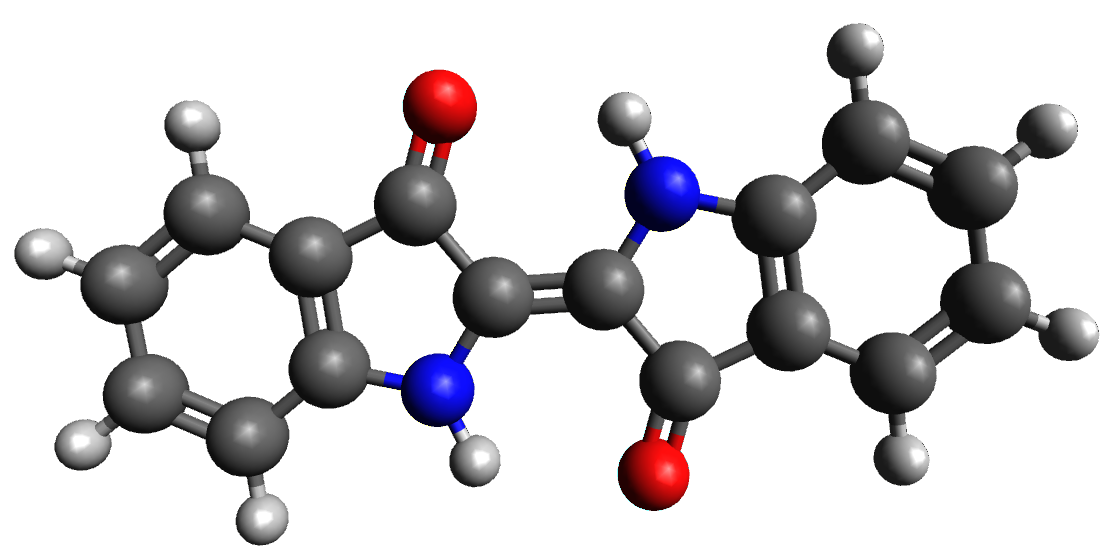
\includegraphics[width=0.6\textwidth]{images/indigo.png}
    \caption{Optimized geometry of indigo on the \ac{TPSS}-D3/def2-SVP level of theory.}
    \label{fig:indigo}
\end{figure}

 The optical transitions of indigo were calculated using time-dependent \ac{HF} method and time-dependent \ac{DFT} methods with the \ac{PBE} and \ac{PBE0} functionals in a def2-SVP basis set. The results are shown in \autoref{tab:indigo_optical_transitions}.


\begin{table}[htbp]
    \centering
    \caption{Optical transition the indigo molecule calculated using different methods in the def2-SVP basis set.}
        \begin{tabular}{@{}lcccc@{}} \toprule
        & HF & PBE & PBE0 & Exp \\
        \midrule
        $\lambda$ (nm) & 373.9 & 618.7 & 533.5 & 610 \\
        Colour & yellow/orange & blue & violet & blue \\
        \bottomrule
        \end{tabular}
        \label{tab:indigo_optical_transitions}
\end{table}

The \ac{PBE} and \ac{PBE0} methods yield a blue and violet color, respectively, while \ac{HF} yields a yellow/orange color. The experimental value is in good agreement with the \ac{PBE} method.

The \ac{PBE0} method is not in agreement with the experimental value. The \ac{HF} method also does not match the experimental valuea and has even more significant deviations than \ac{PBE0}. This indicates that the \ac{HF} method is not suitable for the calculation of optical transitions of indigo at all.

The \ac{PBE} method is a GGA functional that should perform worse than the hybrid \ac{PBE0} functional according to \textit{Jacob's Ladder}, but in this case it yields a better result.

\clearpage
\subsection{NMR Parameters}

\subsubsection*{$^\mathbf{13}$C NMR Shifts for Organic Compounds}

The $^{13}$C NMR shifts for several organic compounds were calculated using the PBEh-3c method for geometry optimization and the PBE/pcSeg-2 method for the calculation of the shielding tensors in ORCA 5.0.4\autocite{Neese2012,Neese2022}. The Lewis structures of the compounds are shown in \autoref{fig:nmr_compounds}. 

\begin{figure}[htbp]
    \centering
    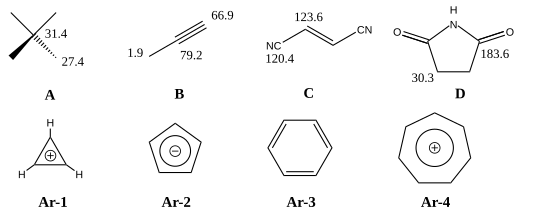
\includegraphics[width=0.9\textwidth]{images/nmr_compounds.png}
    \caption{Lewis structures of four organic compounds A – D with their experimentally obtained chemical shift as well as four aromatic compounds Ar-1 - Ar-4. Figure taken from \cite{AKGrimme2025}.}
    \label{fig:nmr_compounds}
\end{figure}

The chemical shifts were calculated relative to \ac{TMS} and the results are shown in \autoref{tab:nmr_shifts}.


\begin{table}[htbp]
    \centering
    \caption{$^{13}$C chemical shifts ($\delta$) for several organic molecules in reference to \ac{TMS}. Geometries were optimized using PBEh-3c and shielding tensors were calculated at the PBE/pcSeg-2 level of theory.}
    \label{tab:nmr_shifts}
    \begin{tabular}{@{}lcccc@{}} \toprule
        Compound & & \multicolumn{3}{c}{$\delta$ (ppm)} \\
        \midrule
        \multirow{2}{*}{A} & Calc & 34.5 & 34.0  &          \\
                           & Exp  & 27.4 & 31.4   &         \\ \midrule
        \multirow{2}{*}{B} & Calc & 4.03  & 71.2 & 85.4            \\
                           & Exp  & 1.9   & 66.9 & 79.2           \\ \midrule
        \multirow{2}{*}{C} & Calc & 124.0 & 127.9   &        \\
                           & Exp  & 120.4 & 123.6  &        \\ \midrule
        \multirow{2}{*}{D} & Calc & 33.9  &  182.3   &        \\
                           & Exp  & 30.3 & 183.6       &    \\
        \bottomrule
    \end{tabular}
\end{table}

The \ac{MD} and \ac{MAD} values for the chemical shifts of the organic compounds are:

\begin{equation*}
    \text{MD} = \frac{1}{N} \sum_{i=1}^{N} (\delta_{\text{calc}} - \delta_{\text{exp}}) = 4.00 \text{ ppm}
\end{equation*}

\begin{equation*}
    \text{MAD} = \frac{1}{N} \sum_{i=1}^{N} |\delta_{\text{calc}} - \delta_{\text{exp}}| = 4.33 \text{ ppm}.
\end{equation*}

The similarity of the \ac{MD} and \ac{MAD} values indicates that the method has a general difference in the chemical shifts, but the deviations are not too large. The largest deviation is for compound A, which has a difference of 7.1~ppm, and the smallest deviation is for compound D, which has a difference of -1.3~ppm.

The aromatic compounds Ar-1 - Ar-4 were also calculated using the PBE/pcSeg-2 method and their chemical shifts are shown in relation to their $\pi$-electron density $\rho_\pi$ in \autoref{fig:shifts_electron_density}. The chemical shifts were calculated relative to \ac{TMS}.

\begin{figure}[htbp]
    \centering
    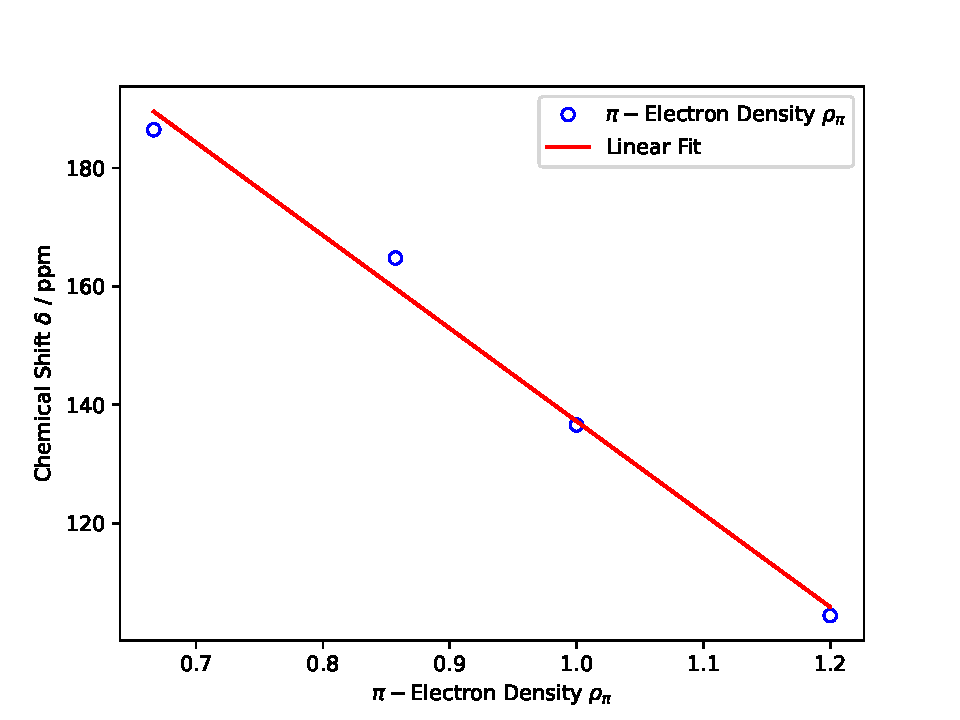
\includegraphics[width=0.8\textwidth]{images/ex8.pdf}
    \caption{Chemical shifts $\delta$ of the aromatic compounds Ar-1 - Ar-4 plotted against the $\pi$-Electron Density $\rho_\pi$. The linear fit is shown as red line and the calculated values as blue circles. The chemical shifts were calculated using the PBE/pcSseg-2 level of theory.}
    \label{fig:shifts_electron_density}
\end{figure}

The chemical shifts of the aromatic compounds show a linear correlation with the $\pi$-electron density, which is expected due to the fact that the chemical shift is influenced by the electron density around the nucleus. The magnetic moment created by the aromatic ring current leads to an increased shielding of the nucleus, which results in a downfield shift of the chemical shift.

\clearpage
\subsubsection*{$^\mathbf{13}$C and $^\mathbf{17}$O NMR Shifts for Acetone}

The effect of the solvent on the NMR shifts of acetone was investigated by calculating the chemical shieldings for acetone in gas-phase and in a solvent (water) using the PBE/pcSeg-2 method. The geometries were optimized in gas-phase and in a solvent using the COSMO model. The chemical shieldings were calculated relative to \ac{TMS} for $^{13}$C and relative to water for $^{17}$O. The results are shown in \autoref{tab:nmr_acetone}.

\begin{table}[htbp]
    \centering
    \caption{Chemical shieldings for Acetone relative to \ac{TMS} ($^{13}$C) and water ($^{17}$O) ($\delta$ in ppm). Reference data was optimized and calculated in gas-phase.}
        \begin{tabular}{@{}lcccccc@{}} \toprule
        \multirow{2}{*}{Geometry} & \multirow{2}{*}{NMR} & \multicolumn{2}{c}{$^{13}$C} & \multicolumn{2}{c}{$^{17}$O} \\
        \cmidrule{3-4} \cmidrule{5-6}
        & & $\delta$ & $\Delta\delta_{\text{gas/gas}}$ & $\delta$ & $\Delta\delta_{\text{gas/gas}}$ \\
        \cmidrule{1-2} \cmidrule{3-4} \cmidrule{5-6}
        Gas & Gas & 214.01 & 0.00 & 672.54 & 0.00 \\
        Gas & Solvent & 224.08 & 10.07 & 616.54 & -60.62 \\
        Solvent & Gas & 216.17 & 2.16 & 682.76 & 10.23 \\
        Solvent & Solvent & 226.25 & 12.24 & 618.83 & -53.71 \\ \bottomrule
        \end{tabular}
    \label{tab:nmr_acetone}
\end{table}

The difference in the chemical shifts for the different combinations of gas-phase and solvent-phase geometries is 2.16~ppm for $^{13}$C and 10.23~ppm for $^{17}$O. In comparison to the absolute value, this gives differences of 1.0-1.5\%. This indicates that the solvent has a significant effect on the chemical shifts of acetone, especially for $^{17}$O. The chemical shift for $^{13}$C is less affected by the solvent, but still shows a significant difference.

The differences in the chemical shifts for gas-phase and solvent-phase for the NMR calculations are larger than that for the geometry. This indicates that the choice for the NMR calculation is more significant than the choice for the geometry.

\clearpage
\subsubsection*{$^\mathbf{1}$H NMR Shifts for Metacyclophane}

The $^{1}$H NMR shifts for in- and out-Metacyclophane were calculated using the PBEh-3c method for geometry optimization and the PBE/pcSeg-2 method for the calculation of the shielding tensors in ORCA 5.0.4\autocite{Neese2012,Neese2022}. The optimized geometries on the PBE-3c method of in- and out-Metacyclophane are shown in \autoref{fig:nmr_metacyclophane}.

\begin{figure}[htbp]
    \centering
    \subfloat[in-Metacyclophane]{
        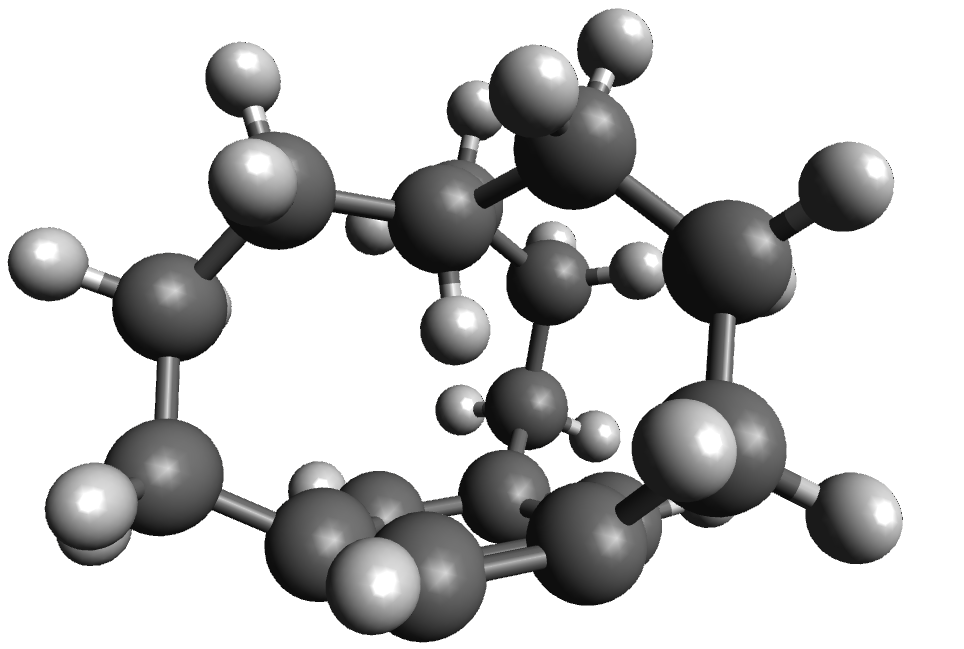
\includegraphics[width=0.48\textwidth]{images/Metacyclophane-In.png}
    }
    \hfill
    \subfloat[out-Metacyclophane]{
        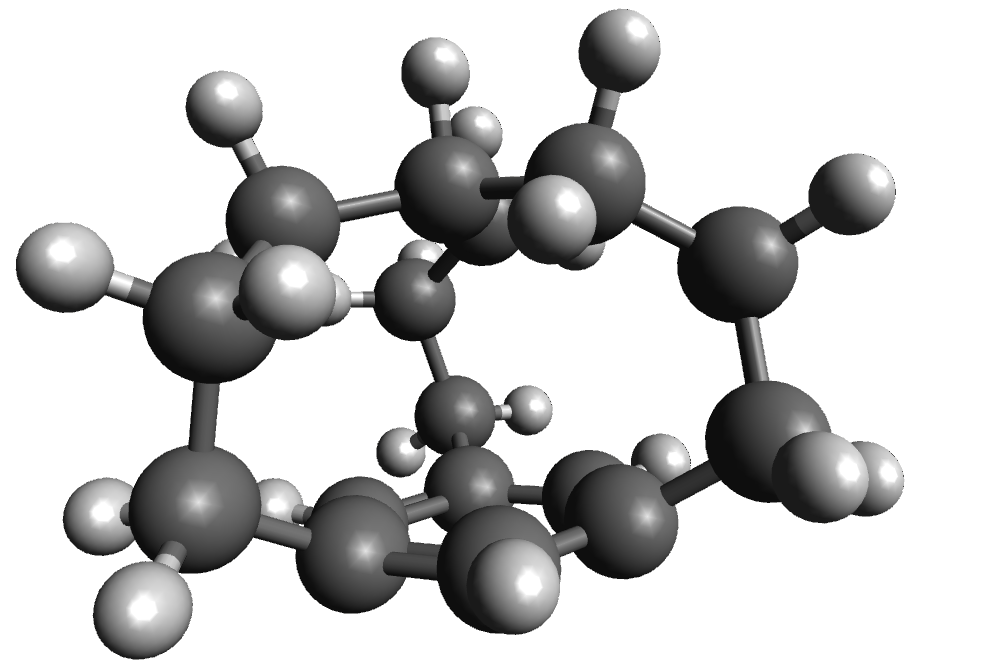
\includegraphics[width=0.48\textwidth]{images/Metacyclophane-Out.png}
    }
    \caption{Optimized geometry of in- and out- [$3^{4,10}$][7]Metacyclophane on the PBE-3c level.}
    \label{fig:nmr_metacyclophane}
\end{figure}

The chemical shifts were calculated relative to \ac{TMS} and are:

\begin{center}
    in: $\delta(^{1}\mathrm{H})$: -3.24

    out: $\delta(^{1}\mathrm{H})$: 2.07.
\end{center}

The chemical shifts for in-Metacyclophane are negative, which indicates that the protons are shielded by the aromatic ring current. The chemical shifts for out-Metacyclophane are positive, which indicates that the protons are deshielded by the aromatic ring current.

\clearpage
\section{Appendix}

\subsection*{Acronyms}

\begin{acronym}
    \acro{B2PLYP}{Becke 2-parameter exchange functional with Perdew-Lee-Yang-Parr correlation functional}
    \acro{B3LYP}{Becke 3-parameter exchange functional with Lee-Yang-Parr correlation functional}
    \acro{BLYP}{Becke-Lee-Yang-Parr}
    \acro{BSIE}{basis set incompleteness error}
    \acro{BSSE}{basis set superposition error}
    \acro{CASSCF}{complete active space self-consistent field}
    \acro{CBS}{complete basis set}
    \acro{CCSD(T)}{coupled cluster with single, double and perturbative triple excitations}
    \acro{DFT}{density functional theory}
    \acro{GSM}{growing string method}
    \acro{HF}{Hartree-Fock}
    \acro{MAD}{mean absolute deviation}
    \acro{MD}{mean deviation}
    \acro{MP2}{Møller-Plesset perturbation theory of second order}
    \acro{PBE}{Perdew-Burke-Ernzerhof}
    \acro{PBE0}{Perdew-Burke-Ernzerhof with 25\% Hartree-Fock exchange}
    \acro{PW6B95}{Perdew-Wang 6-parameter exchange functional with Becke-95 correlation}
    \acro{RHF}{restricted Hartree-Fock}
    \acro{TMS}{tetramethylsilane}
    \acro{TPSS}{Tao-Perdew-Staroverov-Scuseria}
    \acro{UHF}{unrestricted Hartree-Fock}
    \acro{ZPVE}{zero-point vibrational energy}
\end{acronym}

\printbibliography[heading=bibintoc, title={References}] 


\end{document}
